\documentclass[tikz, margin = 2pt]{standalone}
\usetikzlibrary{matrix}
\usetikzlibrary{positioning}
\begin{document}
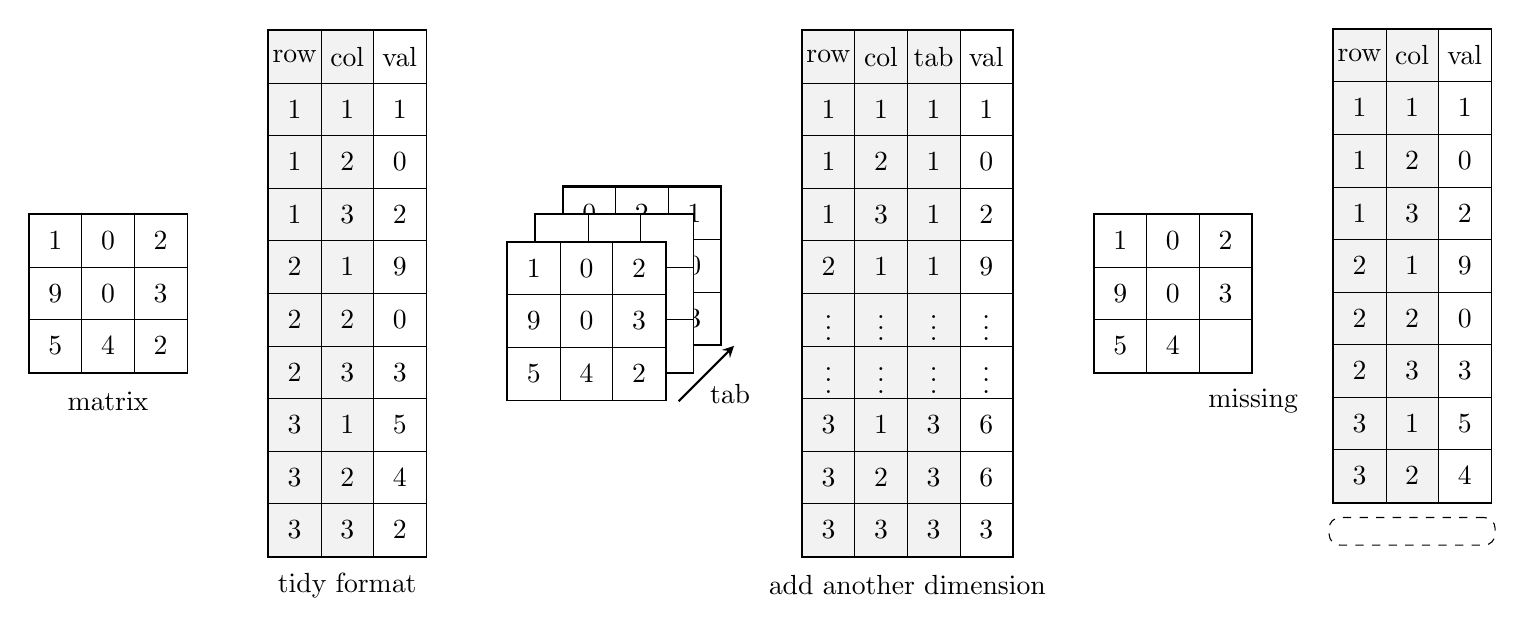
\begin{tikzpicture}[auto matrix/.style={matrix of nodes,
  draw,thick,inner sep=0pt,
  nodes in empty cells,column sep=-0.2pt,row sep=-0.2pt,
  cells={nodes={minimum width=1.9em,minimum height=1.9em,
   draw,very thin,anchor=center,fill=white,
   execute at begin node={}
  }}}] 
 
 \node [auto matrix, draw](raw) at (0,0){
  1 & 0 & 2\\
  9 &0 &3 \\
   5& 4& 2\\
 };
 
\node[yshift = -1em] (labraw) at (raw.south){matrix};
 
  \node [right = of raw, auto matrix, draw, nodes={draw},
  nodes={draw}, column 1/.style={nodes={fill=gray!10}},
   column 2/.style={nodes={fill=gray!10}}] (tidy){
 row  & col & val\\
   1& 1&1\\
   1&2 &0\\
   1& 3&2\\
   2&1 &9\\
   2&2 &0\\
   2&3 &3\\
    3&1 &5\\
   3&2 &4\\
   3&3 &2\\
 };
   \node[yshift = -1em] (labtidy) at (tidy.south){tidy format};
 
  \node [right = of tidy, auto matrix, draw, xshift = 2em, yshift = 1em] (matz){
  0 & 2 & 1\\
  8 &0 &0 \\
   6& 6& 3\\
 };
  \node [right = of tidy, auto matrix, draw, xshift = 1em] (maty){
   & &\\
   & &\\
   & &\\
 };
  \node [right = of tidy, auto matrix, draw, yshift=-1em] (matx){
  1 & 0 & 2\\
  9 &0 &3 \\
   5& 4& 2\\
 };
 
 \node [right = of maty, auto matrix, draw, xshift=1em,
  nodes={draw}, column 1/.style={nodes={fill=gray!10}},
  nodes={draw},  column 2/.style={nodes={fill=gray!10}},
 nodes={draw}, column 3/.style={nodes={fill=gray!10}}](tidy3){
 row  & col & tab& val\\
   1& 1&1&1\\
   1& 2&1&0\\
   1& 3 &1&2\\
      2&1 &1&9\\
  \vdots & \vdots & \vdots & \vdots \\
    \vdots & \vdots & \vdots & \vdots \\
   3&1 & 3 &6\\
   3&2 & 3&6\\
   3&3 & 3 &3\\
 };
  \node[yshift = -1em] (labtidy3) at (tidy3.south){add another dimension};
 
 \draw[thick,-stealth] ([xshift=1ex]matx.south east) -- ([xshift=1ex]matz.south east)
  node[midway,below, xshift = 2ex] {tab};
 
  \node [right = of tidy3, auto matrix, draw](rawm){
  1 & 0 & 2\\
  9 &0 &3 \\
   5& 4& \\
 };
   \node[yshift = -1em] (labm) at (rawm.south east){missing};
   
\node [right = of rawm, auto matrix, draw, yshift = 1em,
  nodes={draw}, column 1/.style={nodes={fill=gray!10}},
  nodes={draw},  column 2/.style={nodes={fill=gray!10}}](tidym){
 row  & col & val\\
   1& 1&1\\
   1&2 &0\\
   1& 3&2\\
   2&1 &9\\
   2&2 &0\\
   2&3 &3\\
    3&1 &5\\
   3&2 &4\\
 };
 
\node[yshift = -1em, draw, rounded corners, dashed, minimum width=6em, minimum height=1em] (mb) at (tidym.south){};
\end{tikzpicture}
\end{document}